\documentclass{article}
% Chinese
% \documentclass[UTF8, nofonts, mathptmx, 12pt, onecolumn]{article}
% \usepackage{xeCJK}
% \setCJKmainfont{SimSun}
\usepackage{amsmath}
\usepackage{amsfonts}
\usepackage{amssymb}
\usepackage{wasysym}
% \usepackage{ctex}
\usepackage{graphicx}
\usepackage{float}
\usepackage{geometry}
\geometry{a4paper,scale=0.8}
\usepackage{caption}
\usepackage{subcaption}
% \newcommand{\oiint}{\mathop{{\int\!\!\!\!\!\int}\mkern-21mu \bigcirc} {}}
\newcommand*{\dif}{\mathop{}\!\mathrm{d}}
\newcommand*{\md}{\mathop{}\!\mathrm{d}}
\newcommand*{\me}{\mathrm{e}}

\usepackage{parskip}
\setlength{\parindent}{0cm}

\usepackage{bm}
\let\Oldmathbf\mathbf
\renewcommand{\mathbf}[1]{\boldsymbol{\Oldmathbf{#1}}}
\let\eqnarray\align

\author{Xiping Hu}
\usepackage{authblk}
\author{Xiping Hu}
\affil{https://hxp.plus/}
\title{Homework for Chapter 4}

\begin{document}
\maketitle

\begin{figure}[H]
  \centering
  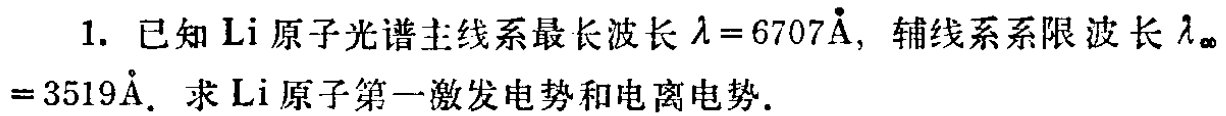
\includegraphics[width=\linewidth]{figures/1}
  \label{fig:}
\end{figure}

\begin{equation*}
  \begin{aligned}
    V_1 = \dfrac{hc}{\lambda e} = 1.850 \  \mathrm{eV} 
  \end{aligned}
\end{equation*}

\begin{equation*}
  \begin{aligned}
    V_{\infty} = \dfrac{hc}{\lambda e} + \dfrac{hc}{\lambda_{\infty} e} = 5.375 \  \mathrm{eV}  
  \end{aligned}
\end{equation*}

\begin{figure}[H]
  \centering
  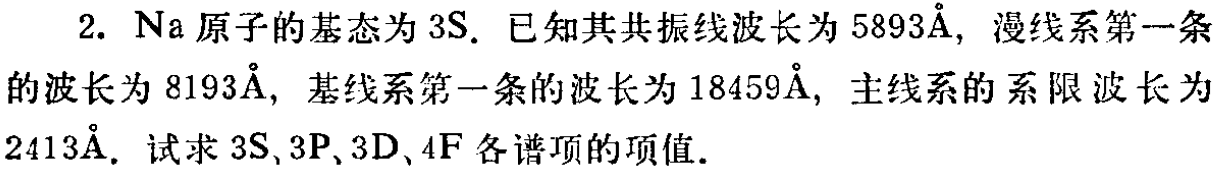
\includegraphics[width=\linewidth]{figures/2}
  \label{fig:}
\end{figure}

\begin{equation*}
  \begin{aligned}
    T_{3S} = \dfrac{1}{\lambda_{p_\infty}} = 4.144 \times 10^6 \  \mathrm{m^{-1}} 
  \end{aligned}
\end{equation*}

\begin{equation*}
  \begin{aligned}
    T_{3P} = \dfrac{1}{\lambda_{p_{\infty}}} - \dfrac{1}{\lambda_{p_{max}}} = 2.447 \times 10^6 \  \mathrm{m^{-1}} 
  \end{aligned}
\end{equation*}

\begin{equation*}
  \begin{aligned}
    T_{3D} = T_{3P} - \dfrac{1}{\lambda_{d_{max}}} = 1.227 \times 10^6 \  \mathrm{m^{-1}}
  \end{aligned}
\end{equation*}

\begin{equation*}
  \begin{aligned}
    T_{4F} = T_{3P} - \dfrac{1}{\lambda_{f_{max}}} = 0.685 \times 10^6 \  \mathrm{m^{-1}} 
  \end{aligned}
\end{equation*}

\begin{figure}[H]
  \centering
  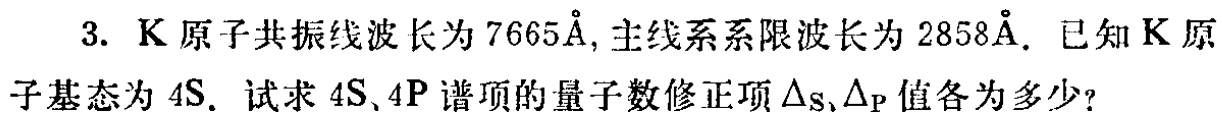
\includegraphics[width=\linewidth]{figures/3}
  \label{fig:}
\end{figure}

\begin{equation*}
  \left\{
  \begin{aligned}
    & T_{4S} = \dfrac{1}{\lambda_{p_{\infty}}} \\
    & T_{4S} = \dfrac{R}{\left( 4 - \Delta_s \right)^2} 
  \end{aligned}
  \right.
\end{equation*}

\begin{equation*}
  \left\{
  \begin{aligned}
    & T_{4P} = \dfrac{1}{\lambda_{p_{\infty}}} - \dfrac{1}{\lambda_{p_{max}}}  \\
    & T_{4P} = \dfrac{R}{\left( 4 - \Delta_p \right)^2} 
  \end{aligned}
  \right.
\end{equation*}

\begin{equation*}
  \left\{
  \begin{aligned}
    \Delta_s = 2.229 \\
    \Delta_p = 1.764
  \end{aligned}
  \right.
\end{equation*}

\begin{figure}[H]
  \centering
  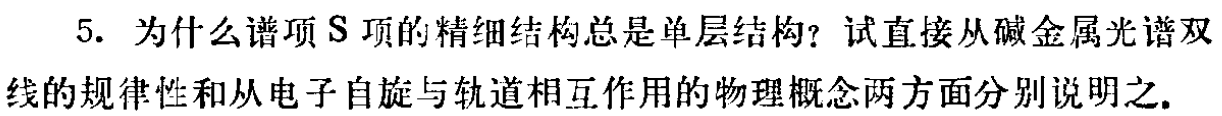
\includegraphics[width=\linewidth]{figures/5}
  \label{fig:}
\end{figure}

Experiments showed that the principal series yellow sodium line 3s-3p is not a simple line but is a doublet. And this phenomenon exists in other alkalis metal atoms. Hence the levels 3p, 4p, 5p, etc, must be double while 3s should be single.

What's more, the angular momentum of the whole electron, including it's self-spin angular momentum and it's orbital momentum, is

\begin{equation*}
  \begin{aligned}
    p_j = \sqrt{j \left( j + 1 \right)} \cdot \dfrac{h}{2 \pi} 
  \end{aligned}
\end{equation*}

Where

\begin{equation*}
  \begin{aligned}
    j &= l \pm \dfrac{1}{2}  
  \end{aligned}
\end{equation*}

When the electron is in s orbital, $l = 0$, since $p_j$ must be real, $j$ cannot be $-\dfrac{1}{2} $. This will cause $p_j$ to be a single value. Which means that the electron can only has one possible direction to self-spin. Which, finally cause the energy level of s orbit to be a single level.

\begin{figure}[H]
  \centering
  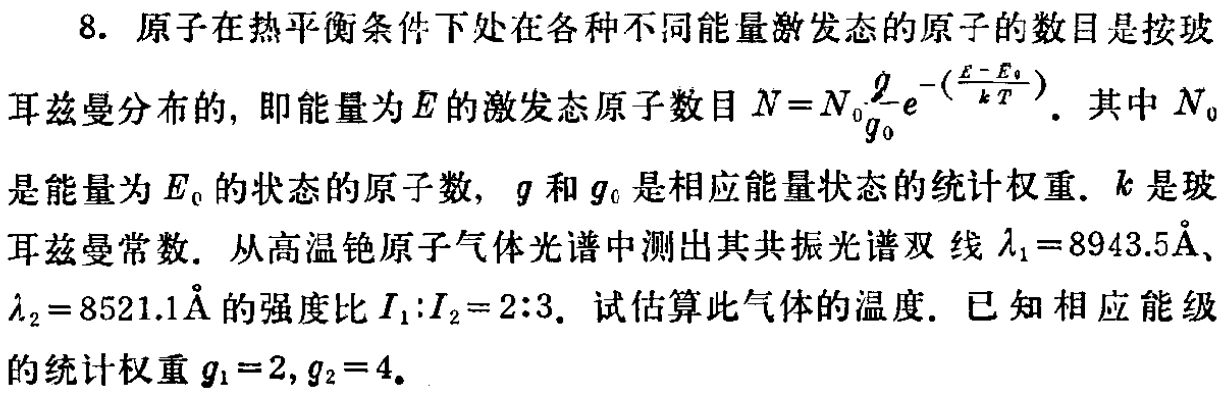
\includegraphics[width=\linewidth]{figures/8}
  \label{fig:}
\end{figure}



\end{document}